\chapter{sel4}
seL4 fa parte della famiglia dei microkernel L4 che risalgono alla prima metà degli anni '90 creato da Jochen Liedtke per sopperire alle scarse performance dei primi sistemi operativi basati su microkernel, ad oggi fa parte del Trustworthy System.\\
Come descritto poco sopra nell'introduzione, seL4 essendo un microkernel, ha un numero di righe di codice sorgente estremamente piccolo e questo è sufficiente per determinare che non è un sistema operativo ma soltanto un microkernel, infatti non fornisce nessun dei servizi che siamo solitamente abituati a trovare su un comune SO, "è solo un sottile involucro attorno all'hardware" \cite{sel4-whitepaper}, tutti i servizi devono essere eseguiti in modalità utente e questi dovranno essere importati ad esempio da sistemi operativi open-source come Linux (oppure scritti da zero). data questa sua definiamola "incapacità" nel fornire servizi all'utente seL4 è anche un \textit{hypervisor}, quindi è possibile eseguire macchine virtuali sulle quali far girare un comune SO che fornirà i servizi non presenti in seL4.\\
\begin{figure}[h]
  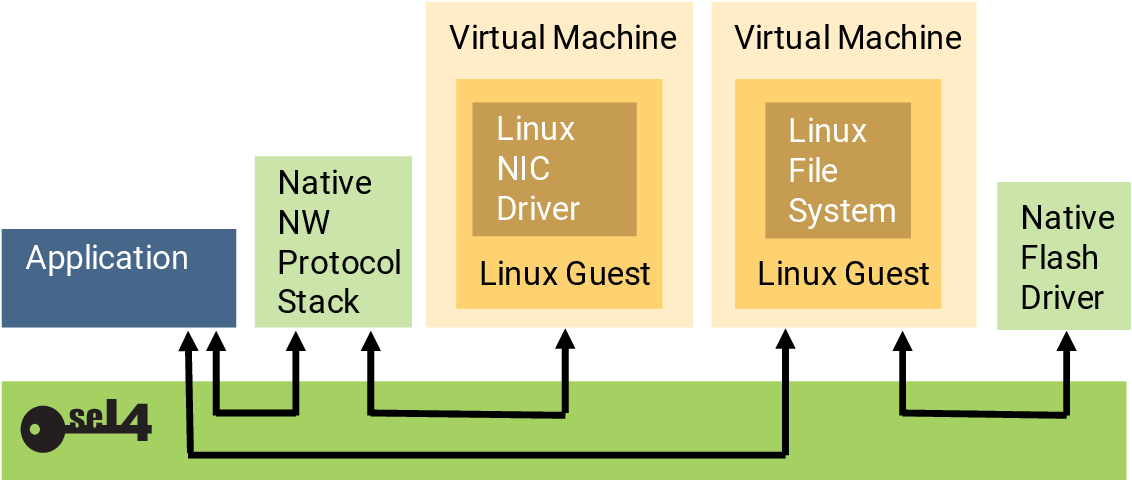
\includegraphics[width=\linewidth]{img/seL4Hypervisor.png}
  \caption{Virtualizzazione del SO Linux per l'intergrazione dei servizi di networking e file system}
  \label{fig:MonolithicVSmicrokernel}
\end{figure}\\

Un esempio pratico può essere quello mostrato in figura 2, in cui è raffigurato seL4, una generica applicazione e due macchine virtuali (VM) sulle quali viene eseguita una versione ridotta al minimo di Linux, che quindi avrà poco più oltre al servizio che dovrà eseguire.
Queste due VM forniranno all'applicazione il servizio di networking ed il file system per la gestione della memoria secondaria (hard disk, supporti rimovibili ecc.), le comunicazioni tra le parti saranno gestite da un canale fornito dal microkernel ma le due macchine virtuali non avranno modo di comunicare tra di loro, non solo questo ma come si vede in figura anche le comunicazioni tra le varie parti e l'applicazione sono ben delineate e precise, nessun'altra comunicazione tra le varie parti è possibile al di fuori di quelle indicate dalle frecce.

\section{capability}
Una \textit{capability} è definita in maniera molto semplice come un riferimento ad oggetto, nel nostro caso specifico possiamo definirli anche come puntatori immutabili, cioè una capability farà sempre riferimento allo stesso oggetto.\\
SeL4 è un sistema capability-based (basato sulle capability) 
questo significa che l'unico modo per eseguire un operazione è attraverso l'invocazione di una capability. Ad ogni capability, inoltre, sono associati dei diritti di accesso, quindi queste sono un incapsulamento di un riferimento ad oggetto e i diritti che sono conferiti ad esso.
ESEMPIO